%!TEX root = doc.tex
\section{Validation}
\label{sec:verification}

To perform a validation of the API, we developed a contract net scenario. This is a deterministic test which uses a fixed data set, thus having always the same outcome. The example was implemented in Repast (using \apiname{}) and then manually ported to JADE, after some adaptations.

\subsection{Experimental Setup}

The diagram in Figure \ref{fig:CNetExample} illustrates the contract net created for this test. An agent (the buyer) intends to purchase a certain quantity of three kinds of goods: rice, flour and oats. Besides the quantities of each product it needs, the buyer also stipulates a maximum price for the whole deal. The buyer will issue a call for proposals (CFP) containing a request for supplies to all agents that announce themselves as suppliers in the DF.

Supplier agents have a maximum supply capacity and a price for each product. After receiving a CFP, the supplier will send to the buyer a PROPOSAL containing a price for each product if the demanded supply is within the seller's capacity. Otherwise, a REFUSE message will be sent to the buyer.
Finally, the buyer agent will compare all valid proposals, choose the cheapest offer for each individual product and reply with an ACCEPT PROPOSAL to the best offers, and REJECT PROPOSAL to all others.

\begin{figure}[h]
	\centering
	\includegraphics[width=3.0in]{figures/CNetExample.pdf}
	\caption{
		Representation of the example contract net.
	}
	\label{fig:CNetExample}
\end{figure}

Using a large data set with values for prices and supply capacity in both frameworks, we ensured the proper comparison of results. For demonstration purposes, we focused on two simple metrics to evaluate our work: time and  outcome. We have run the same experiment with varying numbers of suppliers (as sugested by Figure \ref{fig:performance}) and performed multiple repetitions of each setup.

Time was measured from be begining of the protocol, until all suppliers were notified. The JADE implementation was tested in two different setups: first, with all agents running in a single container; second, with the supplier agents in one container and the buyer in a separate one (but in the same host). In this configuration, all communication between agents happens across containers. All tests were performed using an Intel i7 CPU with 8 logical cores at 2.20 GHz. The second validation metric we used was the actual result of the protocol, i.e who were the supplier agents chosen by the buyer and their price proposals.

\subsection{Results}

For each number of agents, the experiment was run 5 times. The average performance of the experiments is represented in Figure \ref{fig:performance}. As excepted, Repast performance was significantly better, and it excels when the number of agents is high. JADE was able to perform better when using two distinct containers. As studied by Mengistu et. al \cite{mengistu2008scalability}, JADE's performance drops very significantly when there is a high communication-to-computation ratio in the application.

Regarding the outcome of the protocol, as expected the same values were obtained in both implementations, with equal number of suppliers. This allowed us to verify that the behaviour of the protocol is identical in both implementations.


%%%%%%%%%%%%%%%%%%%%%%%%%%%%%%%%%%%%%%%%%%%%%%%
%%%%%%%%%%%%%%%%%% The Chart %%%%%%%%%%%%%%%%%%

\begin{figure}[h]
	\label{fig:performance}
	\centering
	%\includegraphics[width=\linewidth]{figures/performance.png}
	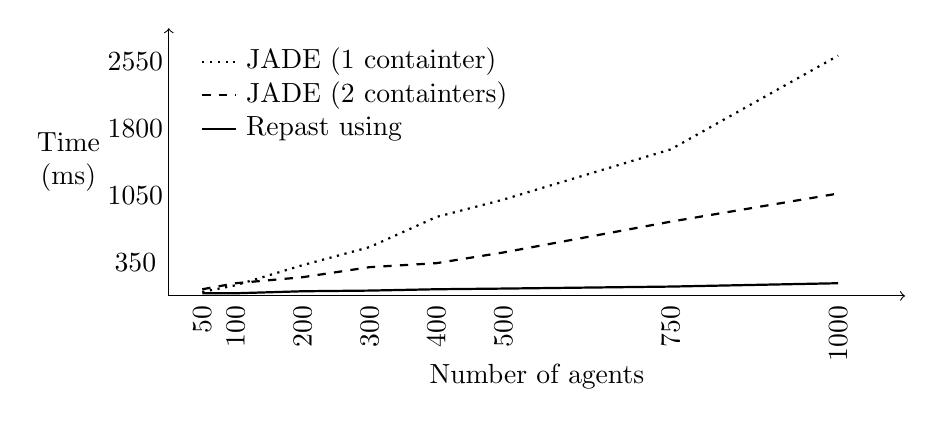
\begin{tikzpicture}[scale=0.85]

		% horizontal axis
		\draw[->] (0,0) -- (11,0);
		\draw (5.5,-1.2) node[align=center] {Number of agents}; %label

		%					  north
		%			west [anchor center] east
		%					  south
		
		% labels
		\draw	(0.5,0) node[rotate=90, anchor=east] {50}
				(1.0,0) node[rotate=90, anchor=east] {100}
				(2.0,0) node[rotate=90, anchor=east] {200}
				(3.0,0) node[rotate=90, anchor=east] {300}
				(4.0,0) node[rotate=90, anchor=east] {400}
				(5.0,0) node[rotate=90, anchor=east] {500}
				(7.5,0) node[rotate=90, anchor=east] {750}
				(10.,0) node[rotate=90, anchor=east] {1000};

		\draw	(-0.5,0.5) node[anchor=center] {350}
				(-0.5,1.5) node[anchor=center] {1050}
				(-0.5,2.5) node[anchor=center] {1800}
				(-0.5,3.5) node[anchor=center] {2550};
		% vertical axis
		\draw[->] (0,0) -- (0,4);
		\draw (-1.5,2) node[align=center] {Time\\(ms)}; %label
		%\draw (-1.5,1.6) node[align=center] {(ms)}; %label

		%% Data %%
		% JADE 2 containers
		\draw[thick,dashed] (0.5,3.0) --
			(1,3.0) node[anchor=west, pos=1.0] {JADE (2 containters)}; %subtitle
		\draw[thick,dashed] (0.5, 0.10) --
					(1.0, 0.19) --
					(2.0, 0.28) --
					(3.0, 0.43) --
					(4.0, 0.49) --
					(5.0, 0.65) --
					(7.5, 1.11) --
					(10., 1.53);
		% JADE 1 containers
		\draw[thick,dotted] (0.5,3.5) --
			(1,3.5) node[anchor=west, pos=1.0] {JADE (1 containter)}; %subtitle
		\draw[thick,dotted] (0.5, 0.06) --
					(1.0, 0.16) --
					(2.0, 0.46) --
					(3.0, 0.73) --
					(4.0, 1.18) --
					(5.0, 1.44) --
					(7.5, 2.19) --
					(10., 3.59);
		% Repast
		\draw[thick] (0.5,2.5) --
			(1,2.5) node[anchor=west, pos=1.0] {Repast using \apiname{}}; %subtitle
		\draw[thick] (0.5, 0.04) --
					(1.0, 0.04) --
					(2.0, 0.07) --
					(3.0, 0.08) --
					(4.0, 0.10) --
					(5.0, 0.11) --
					(7.5, 0.14) --
					(10., 0.19);


	\end{tikzpicture}
	\caption{
		Average execution time of each framework in the different experiments.
	}
\end{figure}

%%%%%%%%%%%%%%%%%%%%%%%%%%%%%%%%%%%%%%%%%%%%%%%
%%%%%%%%%%%%%%%%%%%%%%%%%%%%%%%%%%%%%%%%%%%%%%%
